
\begin{figure}[h]
	\centering
	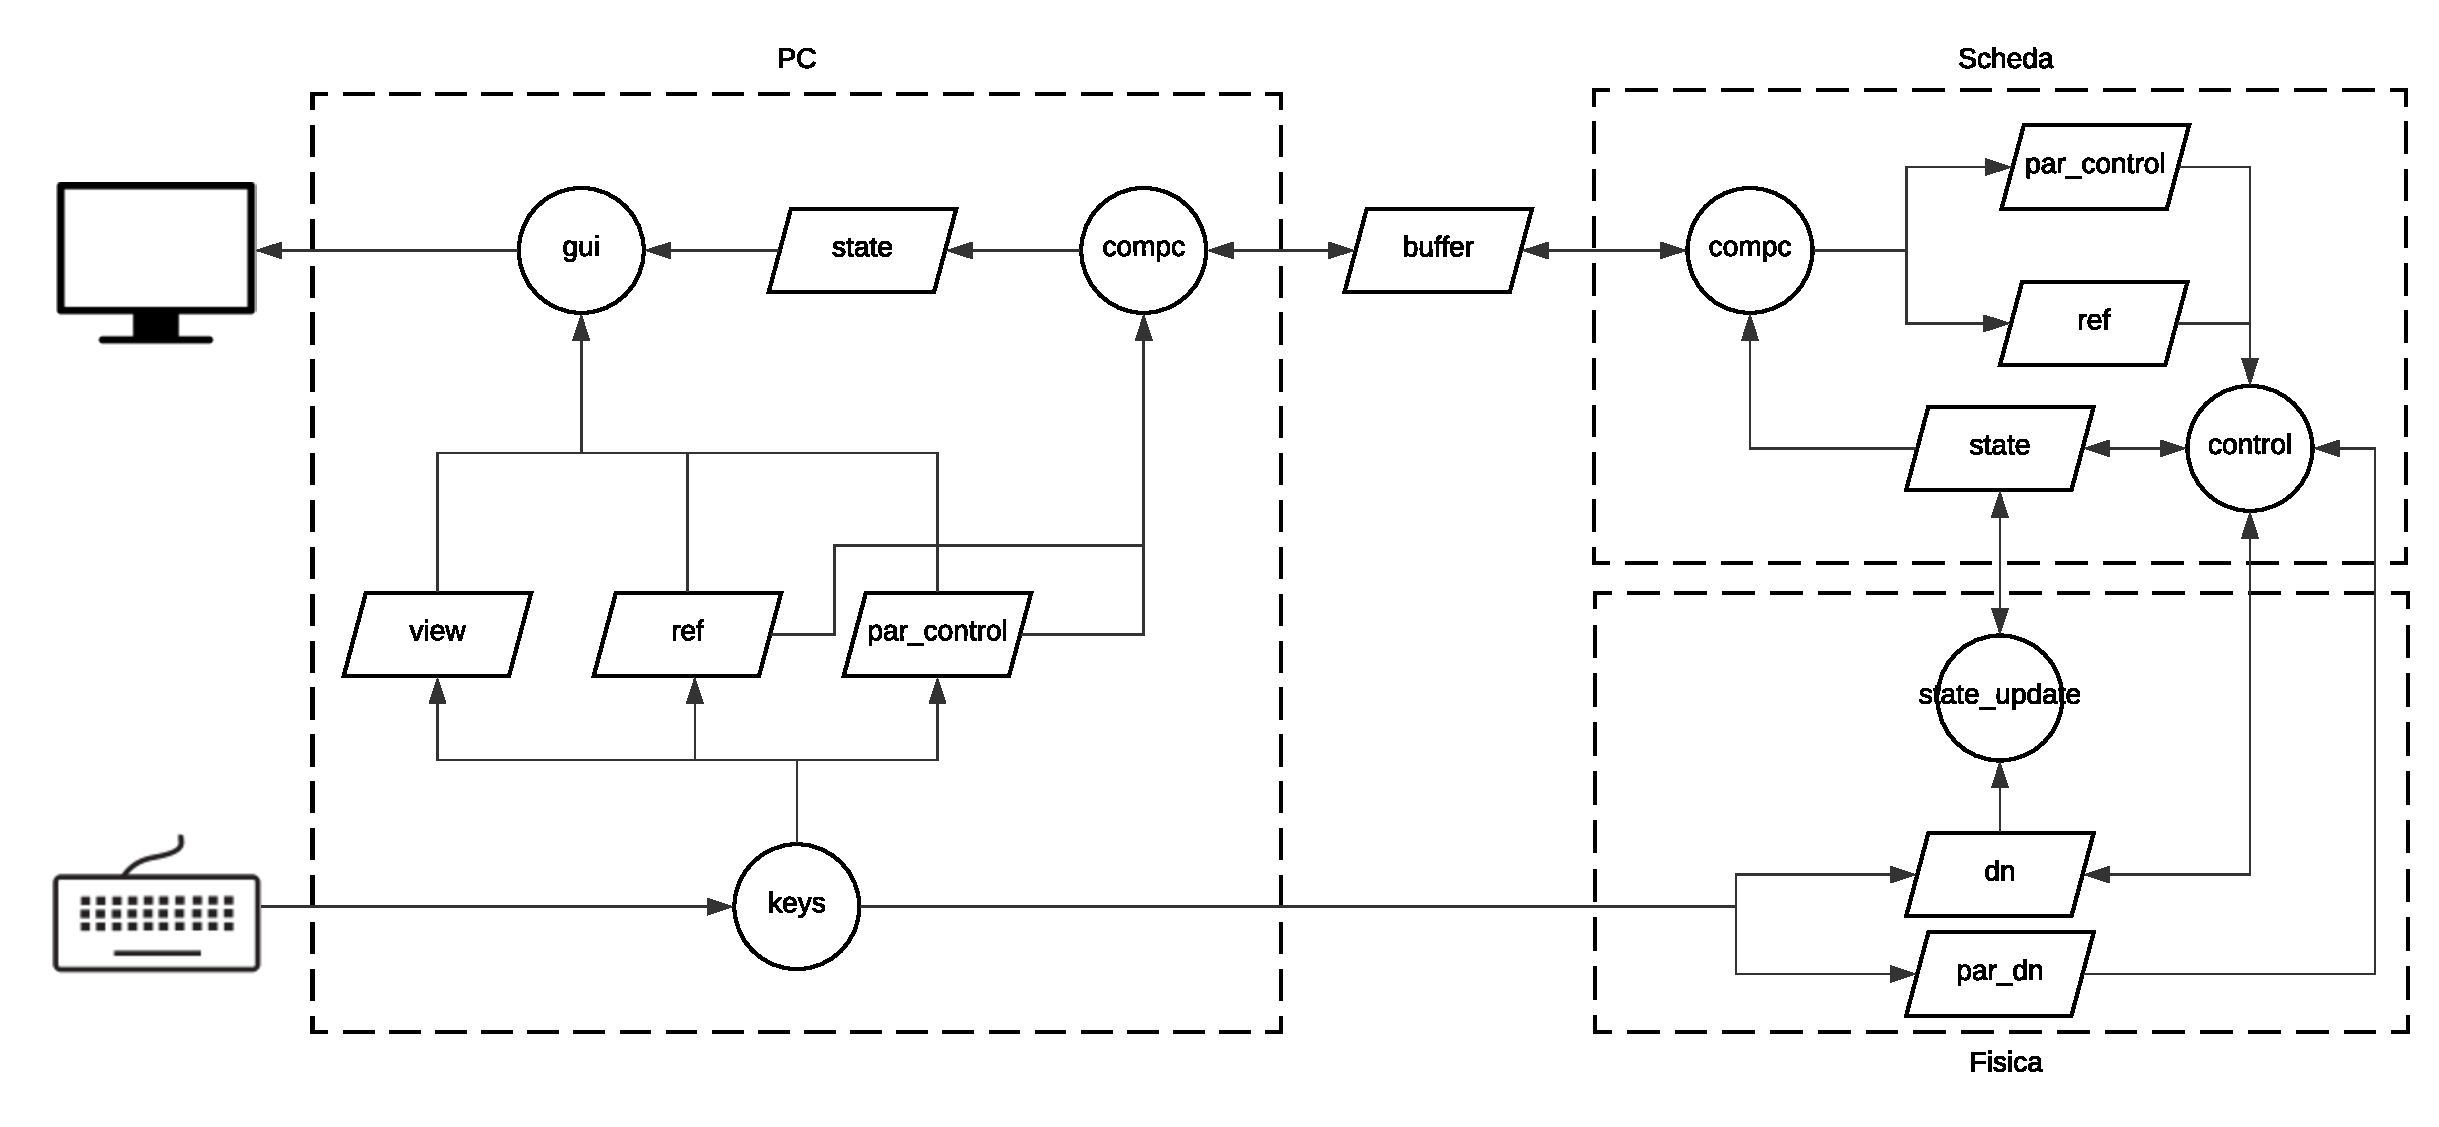
\includegraphics[width=\linewidth]{diagramma_task_risorse.pdf}
	\caption{Diagramma delle risorse e dei task}
	\label{fig:risorse_task}
\end{figure}

L'idea base nella suddivisione dei task \`e stata il voler separare l'interfaccia pc dalla simulazione della scheda e dalla simulazione della fisica del pendolo. A tal proposito sono stati creati i seguenti task:
\begin{itemize}
	\item \textit{state\_update}, aggiorna lo stato in base al modello descritto nella sezione~\ref{sez:modello}
	\item \textit{control}, legge lo stato e il riferimento e modifica l'azione di controllo in base alle leggi sviluppate nella sezione~\ref{sez:controllo}
	\item \textit{comboard}, comunica tra scheda e il buffer condiviso
	\item \textit{compc}, comunica tra pc e il buffer condiviso
	\item \textit{keys}, legge che tasti vengono premuti e compie azioni di conseguenza
	\item \textit{gui}, disegna e aggiorna l'interfaccia utente esposta nella sezione~\ref{sez:interfaccia}
\end{itemize}

\begin{table}[h]
	\centering
	\begin{tabular}{rcc}
		\multicolumn{1}{c}{Task}                & Periodo      & Priorit\`a \\ \hline
		\textit{state\_update} & $\SI{1}{\ms} $  & 99         \\
		\textit{control}      & $\SI{5}{\ms} $ & 90         \\
		\textit{comboard}     & $\SI{5}{\ms} $ & 30         \\
		\textit{compc}        & $\SI{5}{\ms} $ & 30         \\
		\textit{keys}         & $\SI{20}{\ms}$ & 20         \\
		\textit{gui}          & $\SI{40}{\ms}$ & 10         \\ 
	\end{tabular}
\caption{Priopriet\`a task}
\label{tab:info_task}
\end{table}

Per differenziare ulteriormente le simulazioni delle varie componenti \`e stata assegnato un diverso core della CPU ad ogni gruppo di task. Si ha quindi \textit{state\_update} su un processore a lui dedicato, \textit{control} e \textit{comboard} su un secondo e infine \textit{keys}, \textit{compc} e \textit{gui} su un terzo.

\subsubsection{\textit{state\_update}}
Questo task si occupa di simulare la fisica del pendolo. Essendo impossibile eseguire l'aggiornamento dello stato in modo continuo, la velocit\`a di esecuzione \`e molto importante per approssimare in modo appropriato il modello discreto. Per questo motivo \`e il task di maggior priorit\`a e con minore tempo di esecuzione.

La funzione principale di questo task \`e \texttt{physics} ottenuta tramite l'Embedded Coder di \textsc{Simulink--Matlab}.

\subsubsection{\textit{control}}
I suoi scopi sono quelli di simulare le azioni del microcontrollore tramite la funzione \texttt{controller} e quello di aggiornare la structure \texttt{dn} per mezzo della funzione \texttt{disturbance and noise}. 

Le funzioni \texttt{controller} e \texttt{disturbance and noise} sono state ottenute dall'uso dell'Em\-bed\-ded Coder di \textsc{Simulink--Matlab}. La prima, con le opportune modifiche, \`e la funzione da caricare sul microcontrollore stesso. La priorit\`a di \textit{control} \`e secondaria solo alla simulazione fisica.

\subsubsection{\textit{compc} e \textit{comboard}}
Questi sono i due task di comunicazione, \textit{compc} lato pc e \textit{comboard} lato scheda. Il primo si occupa di scrivere il riferimento e i vari parametri di controllo sul buffer e di leggere lo stato del pendolo in memoria sul buffer. Il secondo in modo opposto, legge il riferimento e i parametri di controllo e scrive lo stato.

\subsubsection{\textit{keys}}
Si occupa delle varie interazioni tra tastiera e le strutture dati a cui ha accesso il pc. I vari tasti che modificano riferimento, parametri e vista sono visibili nell'interfaccia accanto alla variabile che vanno a modificare e in basso per i tasti di reset.

\subsubsection{\textit{gui}}
Scrive su schermo tutte le statistiche relative ai task, i parametri, i riferimenti e lo stato. Inoltre si occupa di disegnare le varie viste descritte nella sezione~\ref{sez:interfaccia}. 

A differenza dei precedenti questo task non \`e coinvolto nella simulazione del pendolo, la sua esecuzione \`e quindi secondaria e il suo periodo pu\`o essere rilassato fino a valori che siano sufficienti a visualizzare le informazioni su schermo senza troppa latenza. Il periodo \`e stato quindi scelto per avere 25 frame al secondo.
















